\documentclass[a4paper,14pt]{article} % формат документа

\usepackage{cmap} % поиск в ПДФ
\usepackage[T2A]{fontenc} % кодировка
\usepackage[utf8]{inputenc} % кодировка исходного текста
\usepackage[english,russian]{babel} % локализация и переносы
\usepackage[left = 2cm, right = 1cm, top = 2cm, bottom = 2 cm]{geometry} % поля
\usepackage{listings}
\usepackage{graphicx} % для вставки рисунков
\usepackage{amsmath}
\usepackage{float}
\graphicspath{{pictures/}}
\DeclareGraphicsExtensions{.pdf,.png,.jpg}
\newcommand{\anonsection}[1]{\section*{#1}\addcontentsline{toc}{section}{#1}}

\lstset{ %
	language=Python,                % Язык программирования 
	numbers=left,                   % С какой стороны нумеровать          
	frame=single,                    % Добавить рамку
}

\begin{document}
	\begin{titlepage}

       		\begin{center}
         		\large
		
        			Государственное образовательное учреждение высшего профессионального образования\\
       			“Московский государственный технический университет имени Н.Э.Баумана”
         		\vspace{3cm}
            
            		\textsc{Дисциплина: Анализ алгоритмов}
           		\vspace{0.5cm}
                
            		\textsc{Лабораторная работа № 6}
           		 \vspace{3cm}
            
           		 \LARGE 
		 
		 	Муравьиный алгоритм, решение задачи коммивояжера
           		 \vspace{3cm}
            
            		\begin{flushright}
            			Студент: \\
				Сиденко Анастасия Генадьевна \\   
            			Группа: й7-53Б \\
           			\hfill
            
           			Преподаватели: \\
				Строганов Юрий Владимирович \\
           			Волкова Лилия Леонидовна
            			\vfill
            		\end{flushright}
		
			\large
            		2019 г.
		\end{center}

	\end{titlepage}
    
	\tableofcontents
	
	\newpage
    
	\anonsection{Введение}
	\hfill
	
	 Задача коммивояжера занимает особое место в комбинаторной оптимизации и исследовании операций. Исторически она была одной из тех задач, которые послужили толчком для развития этих направлений. Простота формулировки, конечность множества допустимых решений, но колоссальные затраты на полный перебор до сих пор подталкивают к разработке все новых и новых численных методов. 
	 
	 С точки зрения практического применения, она не представляет интерес. 
	 
	 Куда важнее дополнения задачи для транспорта и логистики, когда несколько транспортных средств ограниченной грузоподъемности должны обслуживать клиентов, посещая их в заданные временные окна. [1]
	
	\hfill
	
	Целью данной работы является создание приложения для наглядного представления работы муравьиного алгоритма и для проведения вычислительных экспериментов. 
	
	\hfill

	В работе ставятся следующие задачи. 
	
	\begin{enumerate}
		\item Изучение существующих методов решения задачи коммивояжера. 
		\item Программная реализация алгоритма оптимизации подражанием муравьиной колонии. 	
		\item Проведение вычислительного эксперимента. 
	\end{enumerate}
		
	\newpage


        \section{Аналитическая часть}
        \hfill
        
        История задачи коммивояжёра насчитывает почти 200 лет: в 1832 г. в Германии была опубликована книга «Коммивояжёр: как он должен вести себя и что должен делать для того, чтобы доставлять товар и иметь успех в своих делах -- советы старого курьера» [2].
        
              
        \subsection{Описание задачи}
        \hfill
        
        Задача коммивояжёра -- одна из самых известных задач дискретной оптимизации. Задача заключается в нахождении самого выгодного маршрута, проходящего через указанные города хотя бы по одному разу с последующим возвратом в исходный город [3].
        
       Постановка задачи коммивояжёра: пусть дана сеть из N городов. Коммивояжёр, выходящий из какого-нибудь города, желает посетить $(N-1)$ других городов и вернуться в изначальный пункт. Расстояния между всеми этими городами известны. Требуется установить, в каком порядке коммивояжёру следует посетить города, чтобы суммарное пройденное расстояние было минимальным.
       
       \subsection{Пути решения}
        
        Для нахождения решения задачи коммивояжёра разработано множество различных алгоритмов. 
        
        Среди них:
        \begin{enumerate}
		\item Метод полного перебора; 
		\item Жадный алгоритм; 
		\item Метод ветвей и границ; 
		\item Метод имитации отжига;
		\item Генетический алгоритм; 
		\item Муравьиный алгоритм.
	\end{enumerate}
	
	В данной работе проводится исследование двух из них: метода полного перебора и муравьиного алгоритма. 
	
	Алгоритм полного перебора осуществляет поиск всех решений путём перебора всех вариантов в количестве $N!$ штук, позволяя получить точное решение задачи. 
	
	Это является главным преимуществом алгоритма, ещё одно достоинство – возможность распараллеливания. Главный недостаток метода полного перебора – временные затраты [3]. 
	
	Муравьиный алгоритм (алгоритм оптимизации подражанием муравьиной колонии) представляет собой имитацию поведения колонии муравьёв в природе. В основе муравьиного алгоритма лежит вероятностный подход к поиску оптимального пути, однако имеют большое значение дополнительные критерии.
	
	Преимуществами алгоритма являются невысокая погрешность найденного решения, низкие временные затраты при работе с графами большой размерности, модифицируемость алгоритма и возможность распараллеливания [3]. 
	
	Алгоритм считается одним из самых эффективных наряду с генетическим и также широко применяется на практике.
	
	\hfill
	
	\textbf{Метод решения задачи коммивояжёра на основании муравьиного алгоритма. } [4]
	
	У муравья есть 3 чувства. 
	
	\begin{enumerate}
		\item Обоняние -- муравей может чуять феромон и его концентрацию на ребре. 
		\item Зрение -- муравей может оценить длину ребра. 
		\item Память -- муравей запоминает посещенные города.  
	\end{enumerate}
	
	При старте матрица феромонов $\tau$ инициализируется равномерно некоторой константой. 
	
	Если муравей k находится в городе i и выбирает куда пойти, то делает это по вероятностному правилу. 
	
	\begin{equation}
	P_{x,y}(t) =  
 	\begin{cases}
  		\frac{\tau_{ij}(t)^{\alpha} \eta_{ij}^{\beta}}{\sum_{\text{q в списке посещенных городов}} \tau_{iq}(t)^{\alpha} \eta_{iq}^{\beta}}, \text{если город j в списке целей}\\
   		0, \text{если город j принадлежит списку посещенных городов}
 	\end{cases}
	\end{equation}
	
	$\alpha, \beta$ -- весовые коэффициенты, которые задают важность феромона и привлекательность ребра. 
	
	Ночью учитываем изменение феромона по формуле 2. 
	
	\begin{equation} \tau (t+1)=\tau_{ij}(t)\cdot(1-\rho)+\Delta\tau_{ij}(t) \end{equation}
	\begin{equation} \Delta\tau_{ij}(t)=\sum_{k=1}^n\Delta \tau_{k,ij}(t) \end{equation}
	
	\begin{equation}
	\Delta \tau_{k,ij}(t) =  
 	\begin{cases}
  		\frac{Q}{L_k}, \text{ребро i,j в маршруте k-ого муравья}\\
   		0, \text{иначе}
 	\end{cases}
	\end{equation}
	
	$L_k$ -- длина маршрута k-ого муравья. 
	
	$\rho$ -- коэффициент испарения феромона. 
	
	$Q$ -- нормировочная константа порядка длины наилучшего маршрута. 
	
        \subsection{Выводы} 
        \hfill
        
        Рассмотрев теорию вопроса, необходимо реализовать данный алгоритм, подобрать необходимые коэффициенты и сравнить результаты с результатами алгоритма полного перебора. 
        
        	\newpage

	\section{Конструкторская часть}
	\hfill
	
	Целью данной работы является: создание приложения для наглядного представления работы муравьиного
алгоритма и проведения вычислительных экспериментов. 
	
		
	\subsection{Функциональная модель}
	
	На рисунке 1 представлена функциональная модель нашей задачи.  
	
	\begin{center}
		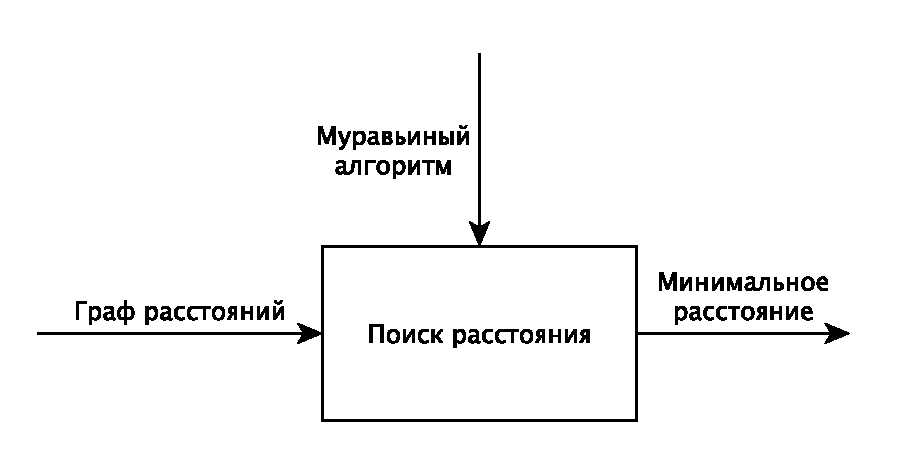
\includegraphics[scale = 0.8]{idef0}
		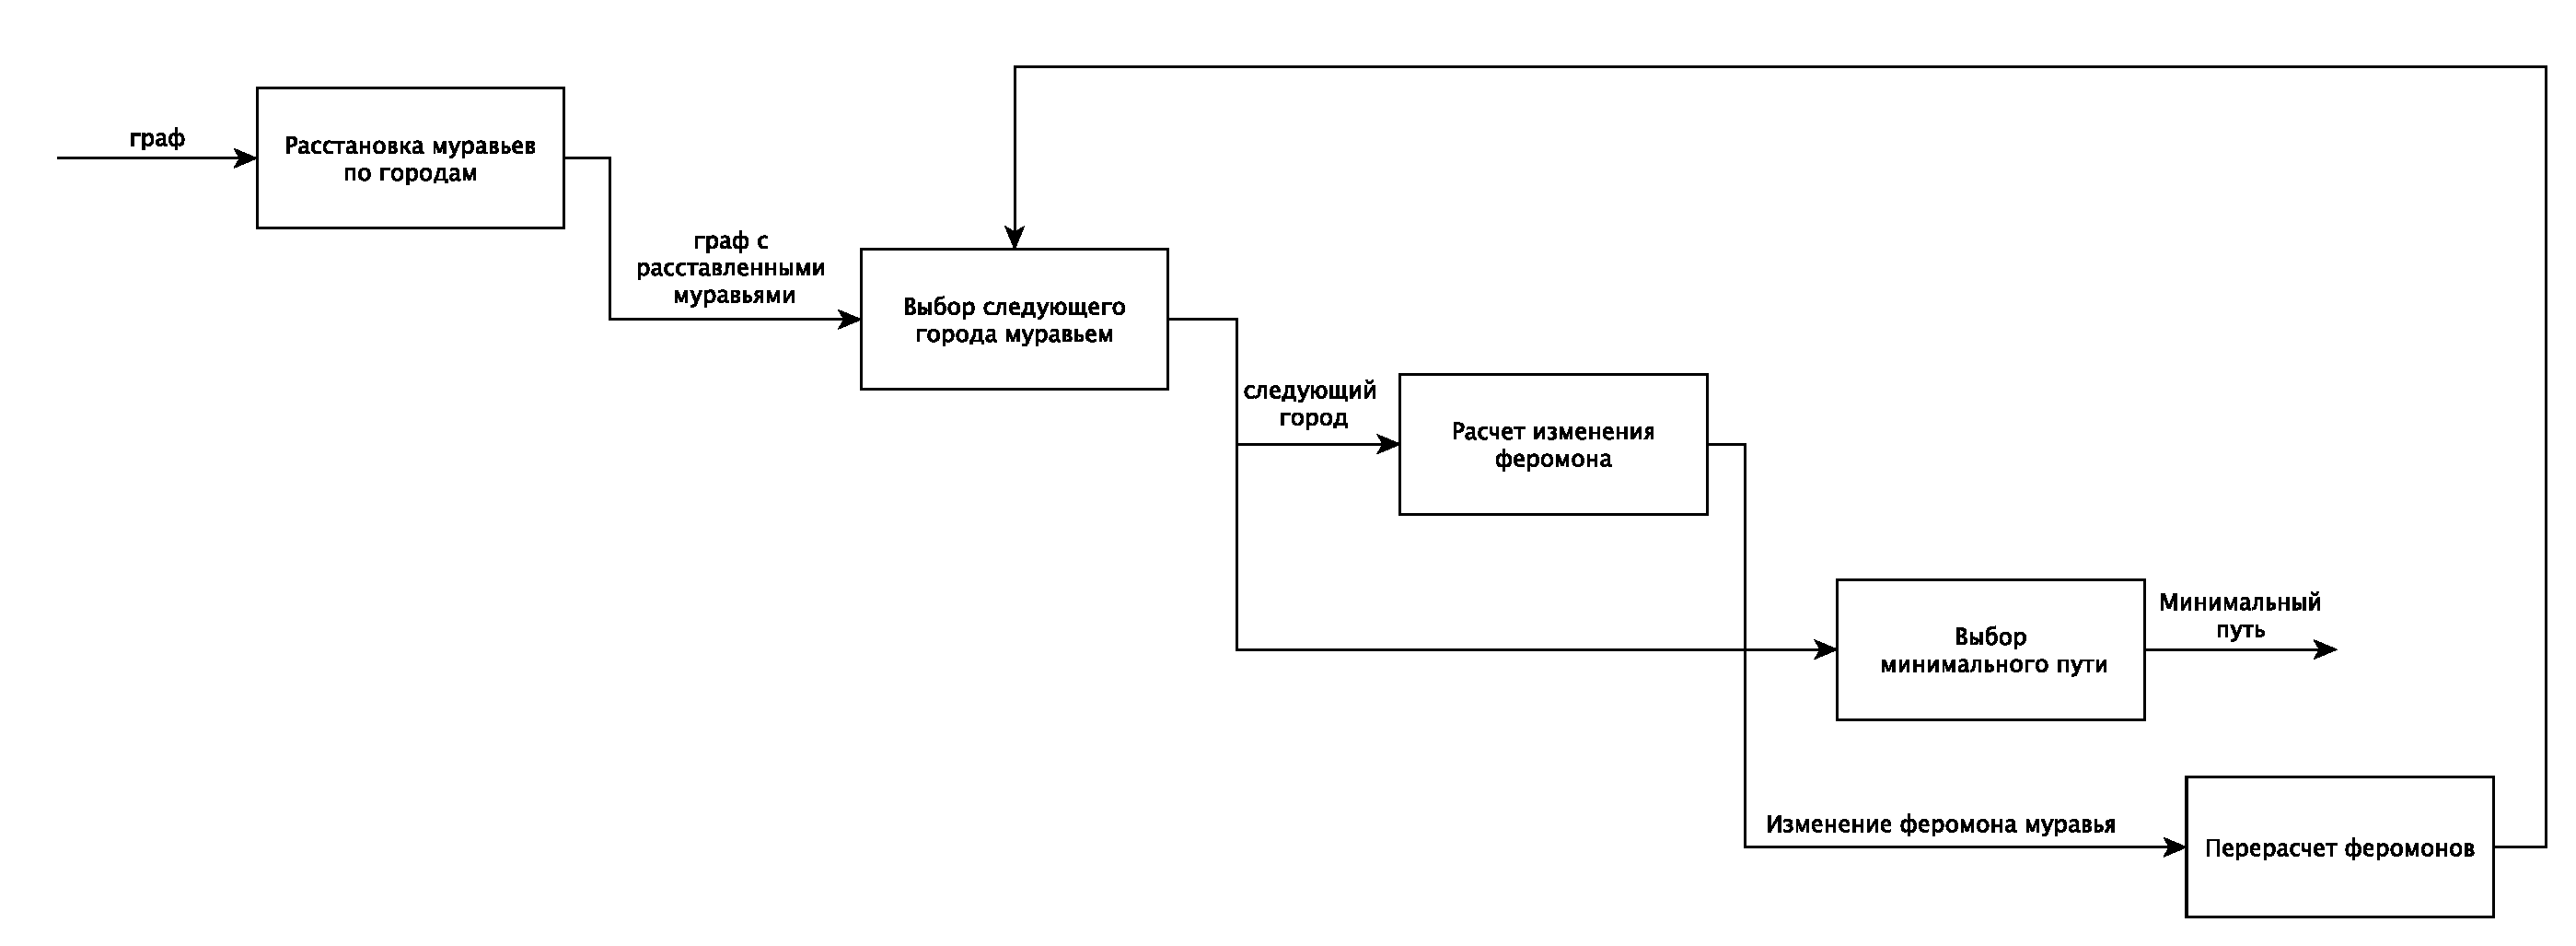
\includegraphics[scale = 0.4]{idef1} \\ Рис.  1 - Функциональная модель муравьиного алгоритма. 
	\end{center}
	        
        \subsection{Схемы алгоритмов}
        \hfill
        
         Приведем схему алгоритма (см. рисунок 2). 
         
        \hfill

	\hfill
	
	\begin{center}
        		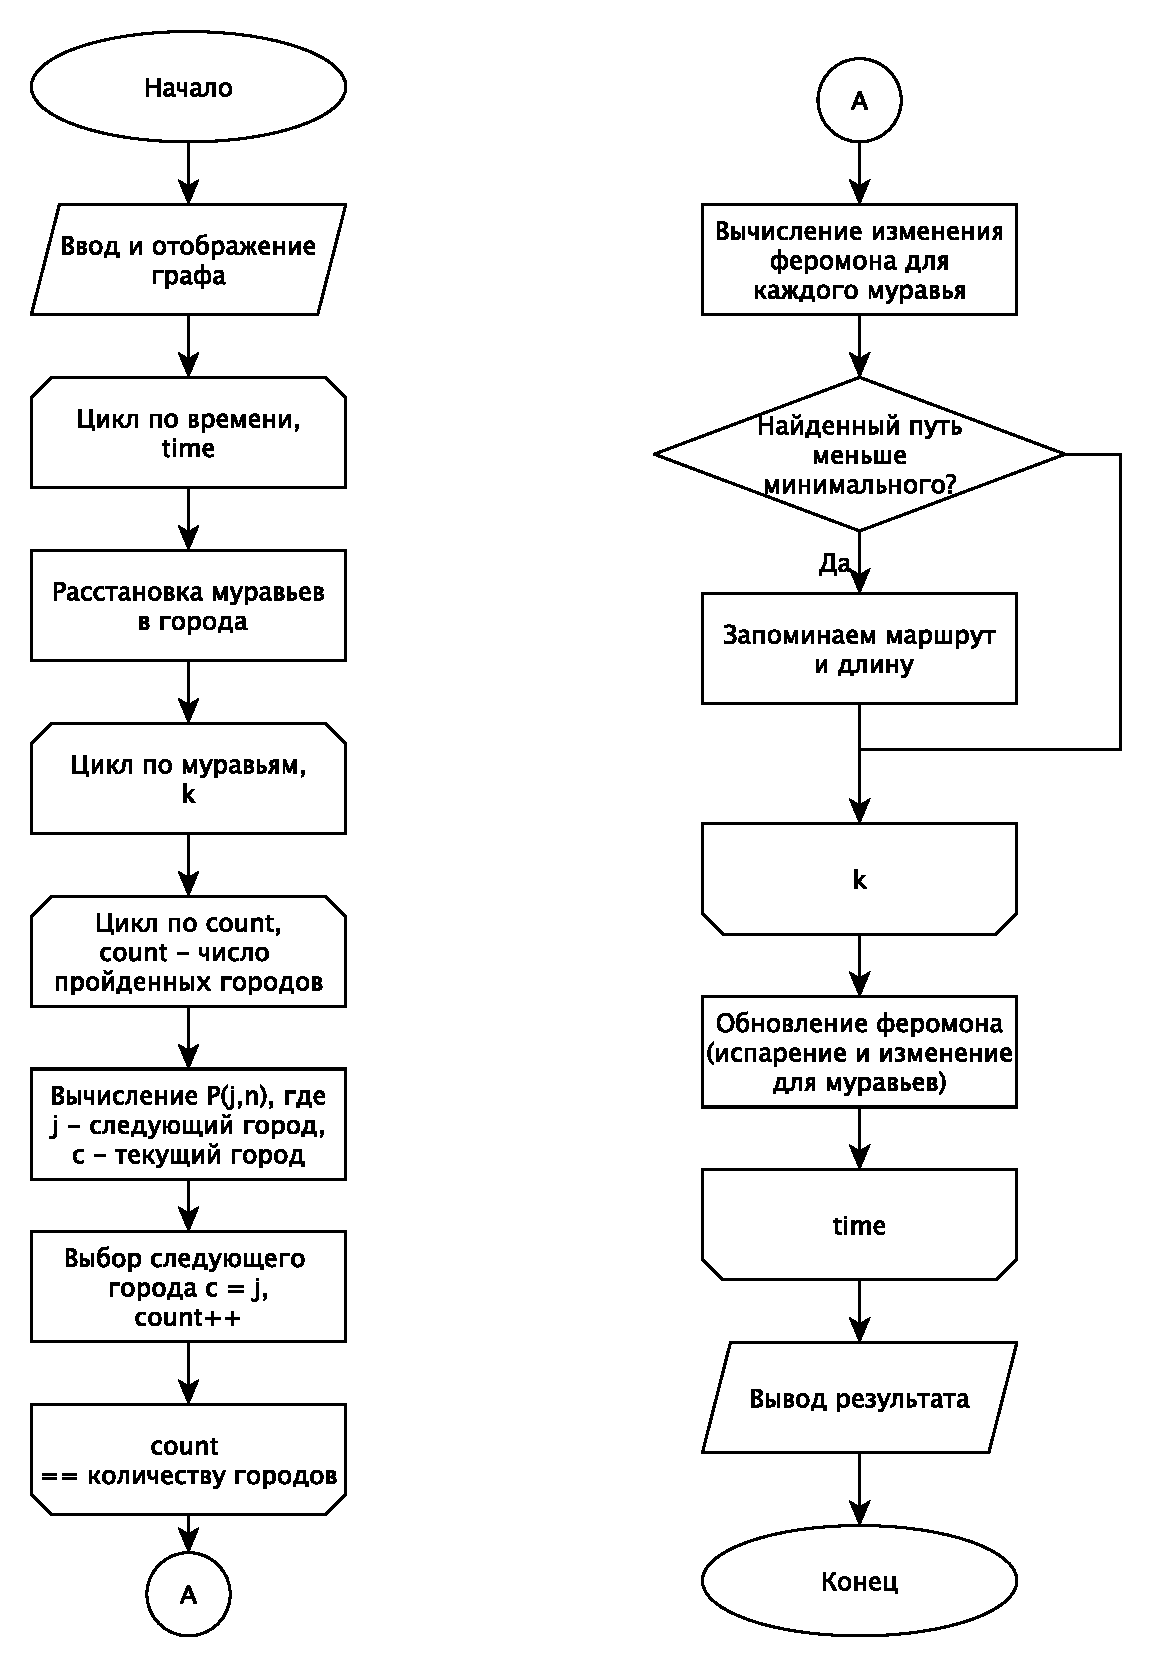
\includegraphics[scale = 0.7]{shema1} \\ Рис. 2 - Алгоритм работы с программы
	\end{center}
        	
	\subsection{Выводы}
	\hfill
	
	Необходимо подобрать коэффициенты, при которых алгоритм будет вычислять реально минимальное расстояние.  
	
			
    	\newpage

        \section{Технологическая часть}
        \hfill
        
        В данном разделе происходит реализация необходимого алгоритма. 
        
         \subsection{Требования к программному обеспечению}
        \hfill
        
        ПО должно предоставлять возможность замеров процессорного времени выполнения реализации каждого алгоритма. Требуется строить графы для различных данных.
        \hfill

        
        \subsection{Средства реализации}
        \hfill
        
        В качестве языка программирования был выбран С++, так как я знакома с этих языком программирования и он удовлетворяет требованиям об использовании dot. [5]
        \hfill
        
        Для генерации случайных чисел использовался метод $rand()$. 
        
        \subsection{Листинг кода}
        \hfill
        
        В листинге 1 представлена реализация муравьиного алгоритма. 
        
        \begin{lstlisting}[caption=Муравьиный алгоритм]
int ant_algorithm(int **matrix, int n, double alpha, double beta, int timemax, double rho) {
  srand(time(NULL));
  double **pheromone = new double * [n];
  for (int i = 0; i < n; i++) {
    pheromone[i] = new double [n];
  }
  for (int i = 0; i < n; i++) {
    for (int j = 0; j < n; j++) {
      pheromone[j][i] = 0.1;
    }
  }
  int minlen = 1000;
  int minway[n];

  for (int time = 0; time < timemax; time++) {
    int *ants = new int [n];
    for (int i = 0; i < n; i++) {
      ants[i] = i + 1;
    }

    double **delta = new double * [n];
    for (int i = 0; i < n; i++) {
      delta[i] = new double [n];
    }

    for (int k = 0; k < n; k++) {
      int count = 0;
      int cities[n];
      for (int i = 0; i < n; i++) {
        cities[i] = 0;
      }
      cities[k] = 1;
      int way[n];
      for (int i = 0; i < n; i++) {
        way[i] = 0;
      }
      way[0] = k;
      int len = 0;

      while (count + 1 < n) {
        double p[n];

        for (int j = 0; j < n; j++) {
          if (0 == cities[j]) {
            p[j] = pow(pheromone[way[count]][j], alpha) * pow(matrix[way[count]][j], 
            								beta);
            double all = 0;
            for (int q = 0; q < count; q++) {
              all += pow(pheromone[way[q]][j], alpha) * pow(matrix[way[q]][j], beta);
            }

            p[j] /= all;
          } else {
            p[j] = 0;
          }
        }
        int arr[n - count - 1];
        int cyc = 0;
        for (int i = 0; i < n; i++) {
          if (0 == cities[i]) {
            arr[cyc] = i;
            cyc++;
          }
        }
        int rdm = rand() % (n - count - 1);
        len += matrix[way[count]][arr[rdm]];
        count++;
        way[count] = arr[rdm];
        cities[arr[rdm]] = 1;
      }
      len += matrix[way[0]][way[n - 1]];

      for (int i = 0; i < n - 1 ; i++) {
        delta[way[i]][way[i + 1]] += minlen / len;
        delta[way[i + 1]][way[i]] += minlen / len;
      }
      if (len < minlen) {
        minlen = len;
        for (int i = 0; i < n; i++)
          minway[i] = way[i];
      }
    }

    for (int i = 0; i < n - 1; i++) {
      for (int j = i + 1; j < n; j++) {
        pheromone[i][j] *= (1 - rho);
        pheromone[i][j] += delta[i][j];
      }
    }
  }

  return minlen;
}
        \end{lstlisting}
	
 	\subsection{Выводы}
	\hfill
	
	Необходимо провести исследовани о выборе коэффициентов в муравьином алгоритме. 
	
	        
        \newpage
        

        \section{Экспериментальная часть}
        \hfill
        
       
        \subsection{Примеры работы}
	\hfill
	
	На рисунке 4 представлены примеры работы программы на разных входных данных. В параметрах командной строки можно указать желаемое число количества чисел, по умолчанию 1.
	\begin{figure}[h]\center
		\begin{tabular}{cc}
			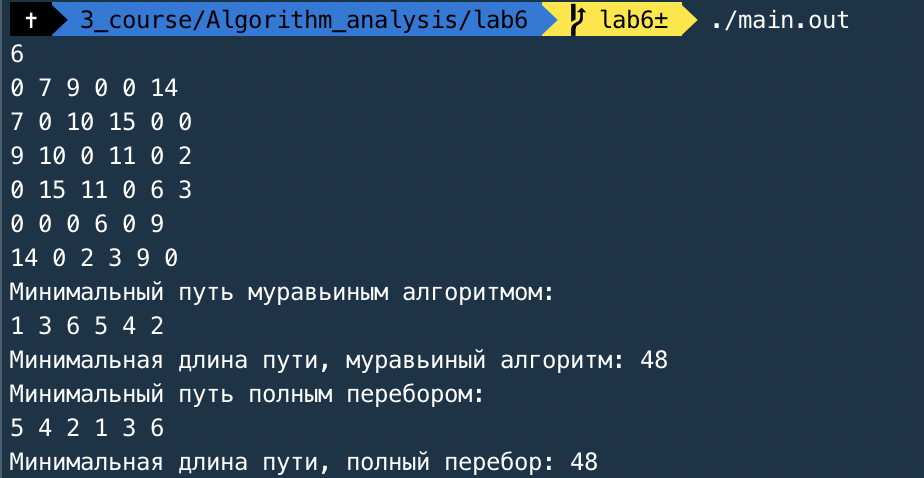
\includegraphics[width=80mm]{ex1} & 
\includegraphics[width=80mm]{ex2} \\
			
\includegraphics[width=80mm]{ex3}
		\end{tabular}
		\\ Рис. 4 - Примеры работы
	\end{figure}
	

	\subsection{Выбор коэффициентов}
	\hfill
	
	Было создано 5 файлов с различными графовыми моделями. 
	
	Проводилось исследование сравнения результата алгоритма полного перебора и муравьиного с различными коэффициентами ($0.2 \le \rho \le 1, 0.2\le\alpha\le1, 0.2\le\beta\le1, 10\le time\le700$). 
	
	$\alpha$ -- коэффициент стадности. 
	
	$\beta$ -- коэффициент жадности. 
	
	time -- количество итераций. 
	
	$\rho$ -- скорость испарения феромонов. 
	
	\hfill
	
	\begin{table}[H]
	\caption{Таблица, соответствующая графу на рисунке 4}
	\begin{tabular}{|c|c|c|c|c|c|}
		\hline
		$\alpha$&$\beta$&time&$\rho$&Длина по алгоритму муравья&Длина по алгоритму полного перебора \\
		\hline
		0.2 &0.2 &10 &0.2 &48 &48\\
		0.2& 0.2 &10 &0.4 &48& 48\\
		0.2 &0.2 &10&0.6 &48 &48\\
		$\cdots$&$\cdots$&$\cdots$&$\cdots$&$\cdots$&$\cdots$\\
		0.8& 0.8& 640& 0.4& 48 &48\\
		0.8 &0.8& 640& 0.6& 48 &48\\
		0.8& 0.8& 640 &0.8 &48& 48\\
		\hline
	\end{tabular}
	\end{table}
	
	\hfill
	
	Представленная таблица 1 соответствует графу на рисунке 4. 
	
	\begin{center}
		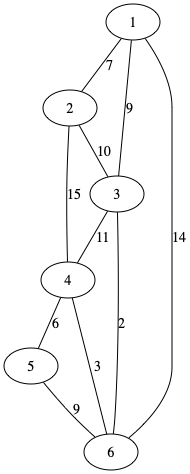
\includegraphics[scale = 0.8]{graph} \\ Рис.  4 - Граф 1, соответствующий тестовым данным 1.  
	\end{center}
	
	Графы представленные на рисунка 5 и 6, вычисляются также при различных значениях. 
	
	\begin{center}
		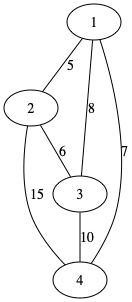
\includegraphics[scale = 0.8]{graph1} \\ Рис.  5 - Граф 2, соответствующий тестовым данным 2.  
	\end{center}
	
	\begin{center}
		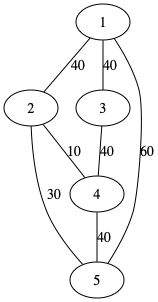
\includegraphics[scale = 0.8]{graph3} \\ Рис.  6 - Граф 3, соответствующий тестовым данным 3. 
	\end{center}
	
	Рассмотрим граф с рисунка 7. 
	
	\begin{center}
		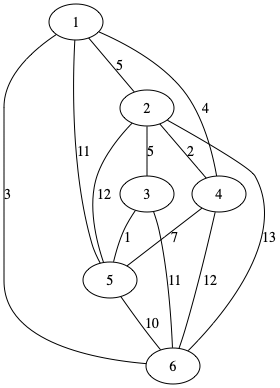
\includegraphics[scale = 0.8]{graph4} \\ Рис.  7 - Граф 4, соответствующий тестовым данным 4.  
	\end{center}
	
	Получим таблицу. 
	
\begin{table}[H]
	\caption{Таблица, соответствующая графу на рисунке 7}
\begin{tabular}{|c|c|c|c|c|c|}
		\hline
		$\alpha$&$\beta$&time&$\rho$&Длина по алгоритму муравья&Длина по алгоритму полного перебора \\
		\hline
0.2&0.2&10&0.2&29&25\\
0.2&0.2&10&0.4&29&25\\
0.2&0.2&10&0.6&29&25\\
0.2&0.2&10&0.8&29&25\\
0.2&0.2&20&0.2&29&25\\
0.2&0.2&20&0.4&29&25\\
0.2&0.2&20&0.6&29&25\\
0.2&0.2&20&0.8&29&25\\
0.2&0.2&40&0.2&25&25\\
0.2&0.2&40&0.4&25&25\\
0.2&0.2&40&0.6&25&25\\
0.2&0.2&40&0.8&25&25\\
0.2&0.2&80&0.2&25&25\\
0.2&0.2&80&0.4&25&25\\
0.2&0.2&80&0.6&25&25\\
0.2&0.2&80&0.8&25&25\\
0.2&0.2&160&0.2&25&25\\
0.2&0.2&160&0.4&25&25\\
0.2&0.2&160&0.6&25&25\\
0.2&0.2&160&0.8&25&25\\
0.2&0.2&320&0.2&25&25\\
0.2&0.2&320&0.4&25&25\\
0.2&0.2&320&0.6&25&25\\
0.2&0.2&320&0.8&25&25\\
0.2&0.2&640&0.2&25&25\\
0.2&0.2&640&0.4&25&25\\
0.2&0.2&640&0.6&25&25\\
0.2&0.2&640&0.8&25&25\\
$\cdots$&$\cdots$&$\cdots$&$\cdots$&$\cdots$&$\cdots$\\
0.8&0.8&10&0.2&29&25\\
0.8&0.8&10&0.4&29&25\\
0.8&0.8&10&0.6&29&25\\
0.8&0.8&10&0.8&29&25\\
0.8&0.8&20&0.2&29&25\\
0.8&0.8&20&0.4&29&25\\
0.8&0.8&20&0.6&29&25\\
0.8&0.8&20&0.8&29&25\\
0.8&0.8&40&0.2&25&25\\
0.8&0.8&40&0.4&25&25\\
0.8&0.8&40&0.6&25&25\\
0.8&0.8&40&0.8&25&25\\
0.8&0.8&80&0.2&25&25\\
0.8&0.8&80&0.4&25&25\\
0.8&0.8&80&0.6&25&25\\
0.8&0.8&80&0.8&25&25\\
0.8&0.8&160&0.2&25&25\\
0.8&0.8&160&0.4&25&25\\
0.8&0.8&160&0.6&25&25\\
0.8&0.8&160&0.8&25&25\\
0.8&0.8&320&0.2&25&25\\
0.8&0.8&320&0.4&25&25\\
0.8&0.8&320&0.6&25&25\\
0.8&0.8&320&0.8&25&25\\
0.8&0.8&640&0.2&25&25\\
0.8&0.8&640&0.4&25&25\\
0.8&0.8&640&0.6&25&25\\
0.8&0.8&640&0.8&25&25\\
\hline
\end{tabular}
\end{table}
Из таблицы 2 видно, что при алгоритм муравья работает при времени (количествах итераций) большим 40. 
	
	
	Рассмотрим граф с рисунка 8. 
	
	\begin{center}
		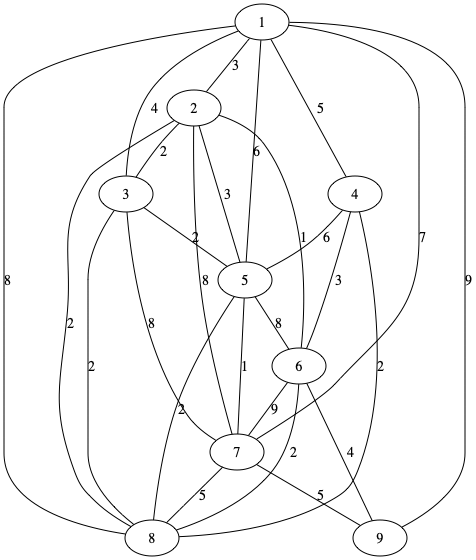
\includegraphics[scale = 0.8]{graph5} \\ Рис.  8 - Граф 5, соответствующий тестовым данным 5.  
	\end{center}
	
	Получим таблицу. 
	
\begin{table}[H]
	\caption{Таблица, соответствующая графу на рисунке 8}
\begin{tabular}{|c|c|c|c|c|c|}
		\hline
		$\alpha$&$\beta$&time&$\rho$&Длина по алгоритму муравья&Длина по алгоритму полного перебора \\
		\hline	
0.2&0.2&10&0.2&43&25\\
0.2&0.2&10&0.4&43&25\\
0.2&0.2&10&0.6&43&25\\
0.2&0.2&10&0.8&43&25\\
0.2&0.2&20&0.2&38&25\\
0.2&0.2&20&0.4&38&25\\
0.2&0.2&20&0.6&38&25\\
0.2&0.2&20&0.8&38&25\\
0.2&0.2&40&0.2&35&25\\
0.2&0.2&40&0.4&35&25\\
0.2&0.2&40&0.6&35&25\\
0.2&0.2&40&0.8&35&25\\
0.2&0.2&80&0.2&30&25\\
0.2&0.2&80&0.4&30&25\\
0.2&0.2&80&0.6&30&25\\
0.2&0.2&80&0.8&30&25\\
0.2&0.2&160&0.2&29&25\\
0.2&0.2&160&0.4&29&25\\
0.2&0.2&160&0.6&29&25\\
0.2&0.2&160&0.8&29&25\\
0.2&0.2&320&0.2&28&25\\
0.2&0.2&320&0.4&28&25\\
0.2&0.2&320&0.6&28&25\\
0.2&0.2&320&0.8&28&25\\
0.2&0.2&640&0.2&26&25\\
0.2&0.2&640&0.4&26&25\\
0.2&0.2&640&0.6&26&25\\
0.2&0.2&640&0.8&26&25\\
$\cdots$&$\cdots$&$\cdots$&$\cdots$&$\cdots$&$\cdots$\\
0.2&0.4&320&0.2&28&25\\
0.2&0.4&320&0.4&28&25\\
0.2&0.4&320&0.6&28&25\\
0.2&0.4&320&0.8&28&25\\
0.2&0.4&640&0.2&26&25\\
0.2&0.4&640&0.4&26&25\\
0.2&0.4&640&0.6&26&25\\
0.2&0.4&640&0.8&26&25\\
$\cdots$&$\cdots$&$\cdots$&$\cdots$&$\cdots$&$\cdots$\\
0.2&0.8&160&0.2&25&25\\
0.2&0.8&160&0.4&25&25\\
0.2&0.8&160&0.6&25&25\\
0.2&0.8&160&0.8&25&25\\
0.2&0.8&320&0.2&25&25\\
0.2&0.8&320&0.4&25&25\\
0.2&0.8&320&0.6&25&25\\
0.2&0.8&320&0.8&25&25\\
0.2&0.8&640&0.2&25&25\\
0.2&0.8&640&0.4&25&25\\
0.2&0.8&640&0.6&25&25\\
0.2&0.8&640&0.8&25&25\\
$\cdots$&$\cdots$&$\cdots$&$\cdots$&$\cdots$&$\cdots$\\
0.4&0.2&160&0.2&25&25\\
0.4&0.2&160&0.4&25&25\\
0.4&0.2&160&0.6&25&25\\
0.4&0.2&160&0.8&25&25\\
0.4&0.2&320&0.2&25&25\\
0.4&0.2&320&0.4&25&25\\
0.4&0.2&320&0.6&25&25\\
0.4&0.2&320&0.8&25&25\\
0.4&0.2&640&0.2&25&25\\
0.4&0.2&640&0.4&25&25\\
0.4&0.2&640&0.6&25&25\\
0.4&0.2&640&0.8&25&25\\
\hline
\end{tabular}
\end{table}

\begin{tabular}{|c|c|c|c|c|c|}
\hline
$\alpha$&$\beta$&time&$\rho$&Длина по алгоритму муравья&Длина по алгоритму полного перебора \\
		\hline	

$\cdots$&$\cdots$&$\cdots$&$\cdots$&$\cdots$&$\cdots$\\
0.6&0.2&10&0.2&31&25\\
0.6&0.2&10&0.4&31&25\\
0.6&0.2&10&0.6&31&25\\
0.6&0.2&10&0.8&31&25\\
0.6&0.2&20&0.2&31&25\\
0.6&0.2&20&0.4&31&25\\
0.6&0.2&20&0.6&31&25\\
0.6&0.2&20&0.8&31&25\\
0.6&0.2&40&0.2&31&25\\
0.6&0.2&40&0.4&31&25\\
0.6&0.2&40&0.6&31&25\\
0.6&0.2&40&0.8&31&25\\
0.6&0.2&80&0.2&31&25\\
0.6&0.2&80&0.4&31&25\\
0.6&0.2&80&0.6&31&25\\
0.6&0.2&80&0.8&31&25\\
0.6&0.2&160&0.2&31&25\\
0.6&0.2&160&0.4&31&25\\
0.6&0.2&160&0.6&31&25\\
0.6&0.2&160&0.8&31&25\\
0.6&0.2&320&0.2&31&25\\
0.6&0.2&320&0.4&31&25\\
0.6&0.2&320&0.6&31&25\\
0.6&0.2&320&0.8&31&25\\
0.6&0.2&640&0.2&29&25\\
0.6&0.2&640&0.4&29&25\\
0.6&0.2&640&0.6&29&25\\
0.6&0.2&640&0.8&29&25\\
$\cdots$&$\cdots$&$\cdots$&$\cdots$&$\cdots$&$\cdots$\\
0.6&0.4&320&0.2&31&25\\
0.6&0.4&320&0.4&31&25\\
0.6&0.4&320&0.6&31&25\\
0.6&0.4&320&0.8&31&25\\
0.6&0.4&640&0.2&29&25\\
0.6&0.4&640&0.4&25&25\\
0.6&0.4&640&0.6&25&25\\
0.6&0.4&640&0.8&25&25\\
$\cdots$&$\cdots$&$\cdots$&$\cdots$&$\cdots$&$\cdots$\\
0.6&0.6&640&0.2&25&25\\
0.6&0.6&640&0.4&25&25\\
0.6&0.6&640&0.6&25&25\\
0.6&0.6&640&0.8&25&25\\
$\cdots$&$\cdots$&$\cdots$&$\cdots$&$\cdots$&$\cdots$\\
0.6&0.8&640&0.4&25&25\\
0.6&0.8&640&0.6&25&25\\
0.6&0.8&640&0.8&25&25\\
$\cdots$&$\cdots$&$\cdots$&$\cdots$&$\cdots$&$\cdots$\\
0.8&0.2&640&0.2&25&25\\
0.8&0.2&640&0.4&25&25\\
0.8&0.2&640&0.6&26&25\\
0.8&0.2&640&0.8&26&25\\
$\cdots$&$\cdots$&$\cdots$&$\cdots$&$\cdots$&$\cdots$\\
0.8&0.8&640&0.4&26&25\\
0.8&0.8&640&0.6&26&25\\
0.8&0.8&640&0.8&26&25\\	
\hline
\end{tabular}

Из таблицы 3 видно, что при алгоритм муравья работает при времени (количествах итераций) большим 160 и коэффициентах $\alpha, \beta $ 0.2, 0.8 или 0.4, 0.2 соотвественно. 

И при итерациях от 640 и $\alpha$ 0.6 и $\beta$ от 0.4. 
 
И при итерациях от 640 и $\alpha$ большем 0.8 и $\beta$ любое. 
 
	\subsection{Выводы}
	\hfill
	
	Таким образом, оптимальные коэффициенты:
	
	\begin{tabular}{|c|c|c|c|c|c|}
	\hline
	$\alpha$&$\beta$&time&$\rho$ \\
	\hline	
	0.2&0.8&>160& любое\\
	0.4&0.2&>160& любое\\
	0.6&0.4&>640& любое\\
	>0.8&любое&>640& любое\\
	\hline
	\end{tabular}
	
	$\alpha$ -- коэффициент стадности. 
	
	$\beta$ -- коэффициент жадности. 
	
	time -- количество итераций. 
	
	$\rho$ -- скорость испарения феромонов. 
	
	\newpage

        \anonsection{Заключение}
        
        \hfill
        
        Таким образом было создано приложения для наглядного представления работы муравьиного
алгоритма и проведен вычислительный эксперимент.  
	
	\hfill

	Выполнены следующие задачи. 
	
	\begin{enumerate}
		\item Изучен существующих методов решения задачи коммивояжера. 
		\item Программно реализован алгоритм оптимизации подражанием муравьиной колонии. 	
		\item Проведен вычислительный эксперимент, определены оптимальные коэффциенты. 
	\end{enumerate}
		
            
 	\newpage

        \begin{thebibliography}{}
		\bibitem{} http://www.math.nsc.ru/LBRT/k5/OR-MMF/TSPr.pdf
		\bibitem{} H. Mueller-Merbach. Zweimal travelling Salesman // DGOR-Bulletin, 1983
		\bibitem{} Левитин А. Алгоритмы: введение в разработку и анализ // М.: Вильямс, 2006. – 575 с.
		\bibitem{} Семинары по анализу алгоритмов. 
		\bibitem{} https://www.graphviz.org
	\end{thebibliography} 

\end{document}
